\subsection*{Teil B: Lineare Funktionen erkennen und zeichnen (30 Minuten)}

\begin{enumerate}[label=\arabic*., resume]

    \item \textbf{Ergänze die Wertetabelle für $y = 2x + 1$:}
    \vspace{0.5cm}

    \begin{center}
        \begin{tabular}{|c|c|c|c|c|c|}
            \hline
            $x$ & -2 & -1 & 0 & 1 & 2 \\
            \hline
            $y$ & $2(-2)+1=-3$ & \phantom{-3} & \phantom{-3} & \phantom{-3} & \phantom{-3} \\
            \hline
        \end{tabular}
    \end{center}

    \vspace{1cm}

    \item \textbf{Bestimme Steigung $m$ und y-Achsenabschnitt $t$:}
    \vspace{0.5cm}

    \begin{tabular}{ll}
        a) $y = 3x + 2$ & $m$ = \underline{\hspace{1.5cm}} $t$ = \underline{\hspace{1.5cm}} \\[2ex]
        b) $y = -2x + 5$ & $m$ = \underline{\hspace{1.5cm}} $t$ = \underline{\hspace{1.5cm}} \\[2ex]
        c) $y = x - 4$ & $m$ = \underline{\hspace{1.5cm}} $t$ = \underline{\hspace{1.5cm}} \\[2ex]
        d) $y = -x + 1$ & $m$ = \underline{\hspace{1.5cm}} $t$ = \underline{\hspace{1.5cm}}
    \end{tabular}

    \vspace{1cm}

    \item \textbf{Zeichne die Gerade $y = x + 2$ in das Koordinatensystem:}
    \vspace{0.5cm}

    \textit{Tipp: Bestimme zuerst zwei Punkte mit der Wertetabelle.}

    \begin{center}
        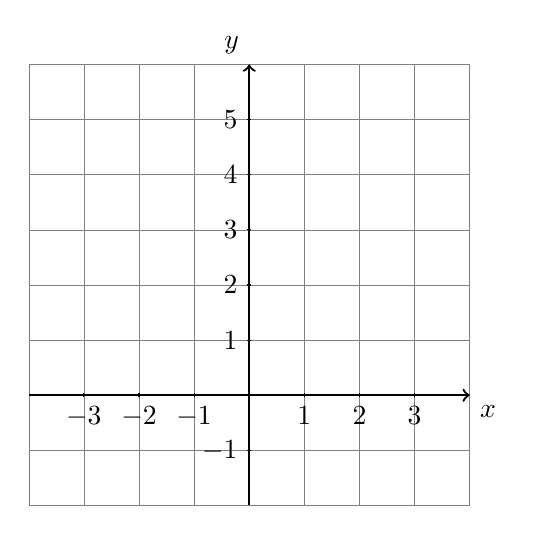
\begin{tikzpicture}[scale=0.7]
            \draw[step=1cm,gray,very thin] (-4,-2) grid (4,6);
            \draw[thick,->] (-4,0) -- (4,0) node[anchor=north west] {$x$};
            \draw[thick,->] (0,-2) -- (0,6) node[anchor=south east] {$y$};
            \foreach \x in {-3,-2,-1,1,2,3}
            \draw (\x cm,1pt) -- (\x cm,-1pt) node[anchor=north] {$\x$};
            \foreach \y in {-1,1,2,3,4,5}
            \draw (1pt,\y cm) -- (-1pt,\y cm) node[anchor=east] {$\y$};
        \end{tikzpicture}
    \end{center}

\end{enumerate}